Studies in the area of Human Factors started during the Second World War, motivated by performance shortfalls and failures related to the operation of equipments used by humans. The studies showed that these problems could diminish when, other than engineering, psychology and physiology were also considered when designing systems that would be handled by human beings \cite{sandom2004human}.

This study area was named "Human Factors" in the United States and "Ergonomics" in Europe. Despite this difference in the names, today they are considered the same field of study. The International Ergonomics Association (IEA) defines Human Factors, therefore Ergonomics, as the following:

\begin{quote}
    \textit{"Ergonomics (or human factors) is the scientific discipline concerned with the understanding of interactions among humans and other elements of a system, and the profession that applies theory, principles, data and methods to design in order to optimize human well-being and overall system performance. Human Factors professionals contribute to the design and evaluation of tasks, jobs, products, environments and systems in order to make them compatible with the needs, abilities and limitations of people"} \cite{karwowski2012discipline}.
\end{quote}

This definition shows that humans and their interaction with systems and devices should be considered during the design process \cite{sandom2004human, sanders1998human, dul2003ergonomics}. This need resulted in the proposal of an ISO Standard: BS EN ISO 13407 "Human-centred design processes for interactive systems". It is essencial to highlight that human-centered design does not mean that the product is designed specifically for an individual. The design has to be suited to everyone, i.e., anyone that may interact with the system \cite{dul2003ergonomics}.

The interaction between humans and machines can be abstracted as illustrated in Figure \ref{fig:human_machine_representaion}. The machine receives inputs from its environment and provides information to the human operator through displays and other monitoring devices. The operator perceives the available information, process it and decides on his/her control actions. Based on the environment's inputs and operator's commands, the machine defines its outputs to the environment.

\begin{figure}[!htb]
    \centering

    \tikzstyle{arrow} = [rounded corners, line width = 1mm, bend left = 15, ->]
    
    \resizebox{0.85\width}{!}{
    \begin{tikzpicture}[node distance=1cm]
        
        \node (information) {
\includegraphics[width=.15\textwidth]{Fundamentação/Fatores Humanos/thinking.png}} 
        node(t_information)[below of = information,yshift=-0.75cm] {Information}
        node(t_information2)[below of = t_information,yshift=0.25cm] {processing};
        
        \node (controlling) [right of=information, xshift=5cm, yshift=-3cm] {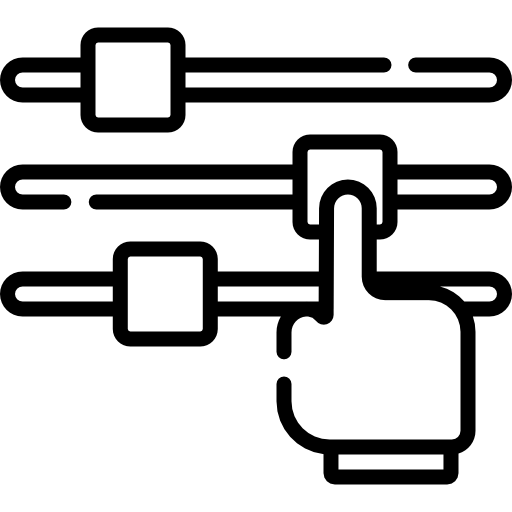
\includegraphics[width=.15\textwidth]{Fundamentação/Fatores Humanos/slider.png}}
        node(t_controlling)[below of = controlling,yshift = -0.75cm] {Controlling};
        
        \node (controls) [below of=controlling, yshift=-5cm,] {
\includegraphics[width=.15\textwidth,angle=90,origin=c]{Fundamentação/Fatores Humanos/control.png}} 
        node(t_controls) [below of = controls, yshift = -0.75cm]{Controls};
        
        \node (machine) [left of=controls, xshift=-5cm, yshift=-2cm] {
\includegraphics[width=.15\textwidth]{Fundamentação/Fatores Humanos/machine.png}} 
        node(t_machine) [below of = machine, yshift = -0.75cm]{Operation};
        
        \node (display) [left of=machine, xshift=-5cm, yshift=2cm] {
\includegraphics[width=.15\textwidth]{Fundamentação/Fatores Humanos/monitor.png}} 
        node(t_display) [below of = display, yshift = -0.75cm]{Display};
        
        \node (senses) [left of=information, xshift=-5cm, yshift=-2cm,] {\begin{tikzpicture}[node distance=1cm]
    \centering
    
    \node (eye) {
\includegraphics[width=.075\textwidth]{Fundamentação/Fatores Humanos/eye.png}};
    
    \node (ear) [right of=eye, yshift=-0.65cm] {
\includegraphics[width=.075\textwidth]{Fundamentação/Fatores Humanos/ear.png}};
    
    \node (nose) [left of=ear, yshift=-0.65cm] {
\includegraphics[width=.075\textwidth]{Fundamentação/Fatores Humanos/nose.png}};
    
    \node (hand) [right of=nose, yshift=-0.85cm] {
\includegraphics[width=.075\textwidth]{Fundamentação/Fatores Humanos/hand.png}};

\end{tikzpicture}} 
        node(t_senses) [below of = senses, yshift = -1.25cm]{Senses};
        
        \node (human) [below of=information, yshift=-4.75cm] {\Large{Human}};
        \node (human) [above of=machine, yshift=3.25cm] {\Large{Machine}};
        \node (human) [above of=information, yshift=1cm] {\Large{Work Environment}};
        
        \node (left_point) [left of=display, xshift=-2, yshift=2.75cm] {};
        \node (right_point) [right of=left_point, xshift=14cm] {};
        
        \node (input) [left of=machine, xshift=-5cm, yshift=-2cm] {\Large{Input}};
        \node (output) [right of=machine, xshift=5cm, yshift=-2cm] {\Large{Output}};
        
    
        \draw [arrow] (information.east) to (controlling.north west);
        \draw [arrow] (t_controlling.south) to (controls.north);
        \draw [arrow] (controls.west) to (machine.east);
        \draw [arrow] (machine.west) to (display.east);
        \draw [arrow] (display.north) to (t_senses.south);
        \draw [arrow] (senses.east) to (information.west);
        \draw [arrow] (input.east) -- (machine);
        \draw [arrow] (machine) -- (output.west);
        \draw [dashed,gray] (left_point) to (right_point);
        
        \draw (-8,-14) rectangle(8cm,1.5cm);
        
    \end{tikzpicture}
    }
    \caption{Human-Machine system representation. Adapted from \cite{sanders1998human}.}
    \label{fig:human_machine_representaion}
\end{figure}

Humans handle devices, machines and equipment during their daily activities. All of these manipulations are susceptible to accidents or failures that can happen because of the interaction between operator, equipment and environment. Each interface with the operator can be a factor. For example:

\begin{itemize}
    \item The operator's body position during an activity: the position can impact the operator's comfort and concentration throughout the activity, therefore, impacting the success rate or the chance of some accident happening  \cite{sanders1998human}.
    
    \item The environment's lighting: illumination can make details more noticeable without provoking discomfort or distraction and even increase productivity  \cite{sanders1998human}.
    
    \item The information displayed and manipulation of the device: the way a information is displayed on a screen, figure or text impacts how efficiently it will be understood by the operator. If this takes too long, it can draw the operator's attention for too long and compromise his/her reaction time.
    
\end{itemize}

Among the various human factors related to human-machine interaction, this work considers mental workload and situation awareness, which are explained in detail in the following sections.